% Options for packages loaded elsewhere
\PassOptionsToPackage{unicode}{hyperref}
\PassOptionsToPackage{hyphens}{url}
%
\documentclass[
]{book}
\usepackage{amsmath,amssymb}
\usepackage{lmodern}
\usepackage{ifxetex,ifluatex}
\ifnum 0\ifxetex 1\fi\ifluatex 1\fi=0 % if pdftex
  \usepackage[T1]{fontenc}
  \usepackage[utf8]{inputenc}
  \usepackage{textcomp} % provide euro and other symbols
\else % if luatex or xetex
  \usepackage{unicode-math}
  \defaultfontfeatures{Scale=MatchLowercase}
  \defaultfontfeatures[\rmfamily]{Ligatures=TeX,Scale=1}
\fi
% Use upquote if available, for straight quotes in verbatim environments
\IfFileExists{upquote.sty}{\usepackage{upquote}}{}
\IfFileExists{microtype.sty}{% use microtype if available
  \usepackage[]{microtype}
  \UseMicrotypeSet[protrusion]{basicmath} % disable protrusion for tt fonts
}{}
\makeatletter
\@ifundefined{KOMAClassName}{% if non-KOMA class
  \IfFileExists{parskip.sty}{%
    \usepackage{parskip}
  }{% else
    \setlength{\parindent}{0pt}
    \setlength{\parskip}{6pt plus 2pt minus 1pt}}
}{% if KOMA class
  \KOMAoptions{parskip=half}}
\makeatother
\usepackage{xcolor}
\IfFileExists{xurl.sty}{\usepackage{xurl}}{} % add URL line breaks if available
\IfFileExists{bookmark.sty}{\usepackage{bookmark}}{\usepackage{hyperref}}
\hypersetup{
  pdftitle={Modelos Matemáticos en Ecología I},
  pdfauthor={Gerardo Martín},
  hidelinks,
  pdfcreator={LaTeX via pandoc}}
\urlstyle{same} % disable monospaced font for URLs
\usepackage{longtable,booktabs,array}
\usepackage{calc} % for calculating minipage widths
% Correct order of tables after \paragraph or \subparagraph
\usepackage{etoolbox}
\makeatletter
\patchcmd\longtable{\par}{\if@noskipsec\mbox{}\fi\par}{}{}
\makeatother
% Allow footnotes in longtable head/foot
\IfFileExists{footnotehyper.sty}{\usepackage{footnotehyper}}{\usepackage{footnote}}
\makesavenoteenv{longtable}
\usepackage{graphicx}
\makeatletter
\def\maxwidth{\ifdim\Gin@nat@width>\linewidth\linewidth\else\Gin@nat@width\fi}
\def\maxheight{\ifdim\Gin@nat@height>\textheight\textheight\else\Gin@nat@height\fi}
\makeatother
% Scale images if necessary, so that they will not overflow the page
% margins by default, and it is still possible to overwrite the defaults
% using explicit options in \includegraphics[width, height, ...]{}
\setkeys{Gin}{width=\maxwidth,height=\maxheight,keepaspectratio}
% Set default figure placement to htbp
\makeatletter
\def\fps@figure{htbp}
\makeatother
\setlength{\emergencystretch}{3em} % prevent overfull lines
\providecommand{\tightlist}{%
  \setlength{\itemsep}{0pt}\setlength{\parskip}{0pt}}
\setcounter{secnumdepth}{5}
\usepackage{booktabs}
\ifluatex
  \usepackage{selnolig}  % disable illegal ligatures
\fi
\usepackage[]{natbib}
\bibliographystyle{apalike}

\title{Modelos Matemáticos en Ecología I}
\author{Gerardo Martín}
\date{2021-08-09}

\begin{document}
\maketitle

{
\setcounter{tocdepth}{1}
\tableofcontents
}
\hypertarget{preuxe1mbulo}{%
\chapter{Preámbulo}\label{preuxe1mbulo}}

\begin{center}
\includegraphics[width=20.83in]{logo} \end{center}

En el curso \textbf{Modelos matemáticos en ecología} aprenderemos a utilizar algunas herramientas matemáticas para entender procesos en ecología. Los contenidos del índice se apegan al \href{Programa-curso.pdf}{programa completo del curso}, el cual se impartirá en los \href{Horario.pdf}{horarios normales establecidos}. Para conocer cuándo, cómo y qué temas se se impartirán puedes consultar la \href{Estrategia-docente.pdf}{estrategia docente}.

\hypertarget{encuadre-de-la-materia}{%
\chapter{Encuadre de la materia}\label{encuadre-de-la-materia}}

\hypertarget{criterios-de-evaluaciuxf3n}{%
\section{Criterios de evaluación}\label{criterios-de-evaluaciuxf3n}}

Las constribuciones a cada calificación parcial serán:

\begin{itemize}
\tightlist
\item
  Asistencia (25\%)
\item
  Trabajos de clase cumplidos (50\%)
\item
  Examen (25\%)
\item
  Participación (2 puntos extra máximo)
\end{itemize}

Cabe señalar, que la asistencia no corresponderá con su presencia en las sesiones sincrónicas, sino con el cumplimiento de los trabajos de clase. La participación se medirá tanto por participación directa en las sesiones sincrónicas como por el seguimiento que uds den a la clase por correo electrónico.

\hypertarget{cuxf3mo-se-daruxe1n-las-clases}{%
\section{¿Cómo se darán las clases?}\label{cuxf3mo-se-daruxe1n-las-clases}}

Trataré de apegarnos a los tiempos de actividades sincrónicas y asincrónicas establecidos en la \href{Estrategia-docente.pdf}{estrategia docente}, pero éstos son completamente flexibles. Una estrategia que me ha funcionado en cursos anteriores ha sido la de dedicar la última actividad sicrónica de la semana a resolver dudas, es en estas sesiones en las que hay muchas posibilidades de conseguir puntos de participación.

Todos los contenidos del curso, lecturas y presentaciones, se irán añadiendo a este sitio web conforme avanza el semestre. En el Google Classroom de la materia se irán anunciando las diferentes actividades y sesiones sincrónicas con anticipación suficiente. Igualmente, los examenes y resultados serán publicados a través de esta plataforma. A petición de uds, también se publicarán aquí los videos de las sesiones sincrónicas que tengamos, en especial para aquellos temas que sean mayor interés/dificultad/importancia. Los trabajos de práctica también se publicarán en Classroom.

\hypertarget{reglas-del-saluxf3n}{%
\section{Reglas del salón}\label{reglas-del-saluxf3n}}

Estas, obviamente, son particulares del modelo en línea, por lo tanto aquí van las reglas de zoom:

\begin{enumerate}
\def\labelenumi{\arabic{enumi}.}
\tightlist
\item
  Micrófonos apagados
\item
  Cámaras prendidas, exceptuando:
  2.1. Si su velocidad de internet lo dificulta
  2.2. Si tienen datos limitados
\item
  Hacer muchas preguntas
\item
  Decirme si paso algo por alto
\end{enumerate}

\hypertarget{contacto}{%
\section{Contacto}\label{contacto}}

Para reportar fallos, resolver dudas y peticiones especiales grupales o individuales por favor enviar correo electrónico a \href{mailto:gerardo.mmc@enesmerida.unam.mx}{\nolinkurl{gerardo.mmc@enesmerida.unam.mx}}.

\hypertarget{unidad-i-introducciuxf3n-a-la-modelaciuxf3n}{%
\chapter{Unidad I: Introducción a la modelación}\label{unidad-i-introducciuxf3n-a-la-modelaciuxf3n}}

\hypertarget{introducciuxf3n-al-concepto-de-modelo-matemuxe1tico}{%
\section{Introducción al concepto de modelo matemático}\label{introducciuxf3n-al-concepto-de-modelo-matemuxe1tico}}

Para comenzar a hablar de modelos matemáticos es preciso tener una idea de por qué las matemáticas forman parte de un grado en ciencias naturales. Los autores \citet{otto2011biologist}, dan cuenta de qué tan comunes son las matemáticas en la labor del biólogo/ecólogo. Hacia el año 2006, una búsqueda sistemática del material publicado en revistas científicas contentiendo la palabra clave ``math'' sugiere que había \textasciitilde900 mil artículos, la mayoría concentrados en revistas especializadas como \emph{Bulletin of Mathematical Biology}, otros en las más prestigiosas \emph{Nature} o \emph{Science}. Una mirada más cercana a las revistas especializadas \emph{Ecology and Evolution} y \emph{American Naturalist} que el 35 y 60\% respectivametne de las publicaciones utilizaron algún modelo matemático para mostrar predicciones. En resumen, la labor de un ecólogo requiere del uso frecuente de matemáticas, si no es mediante el desarrollo de algún modelo, requiere de su entendimiento.

\hypertarget{quuxe9-es-un-modelo}{%
\subsection{¿Qué es un modelo?}\label{quuxe9-es-un-modelo}}

Imaginemos a seis personas invidentes, con la tarea de encontrar qué es el objeto que está frente a ellas usando únicamente el tacto. En la parábola de los seis hombres ciegos, el objeto es un elefante, de modo que la imágen que cada uno de ellos se forma del objeto depende enteramente de la parte del elefante que están tocando.

\begin{figure}

{\centering 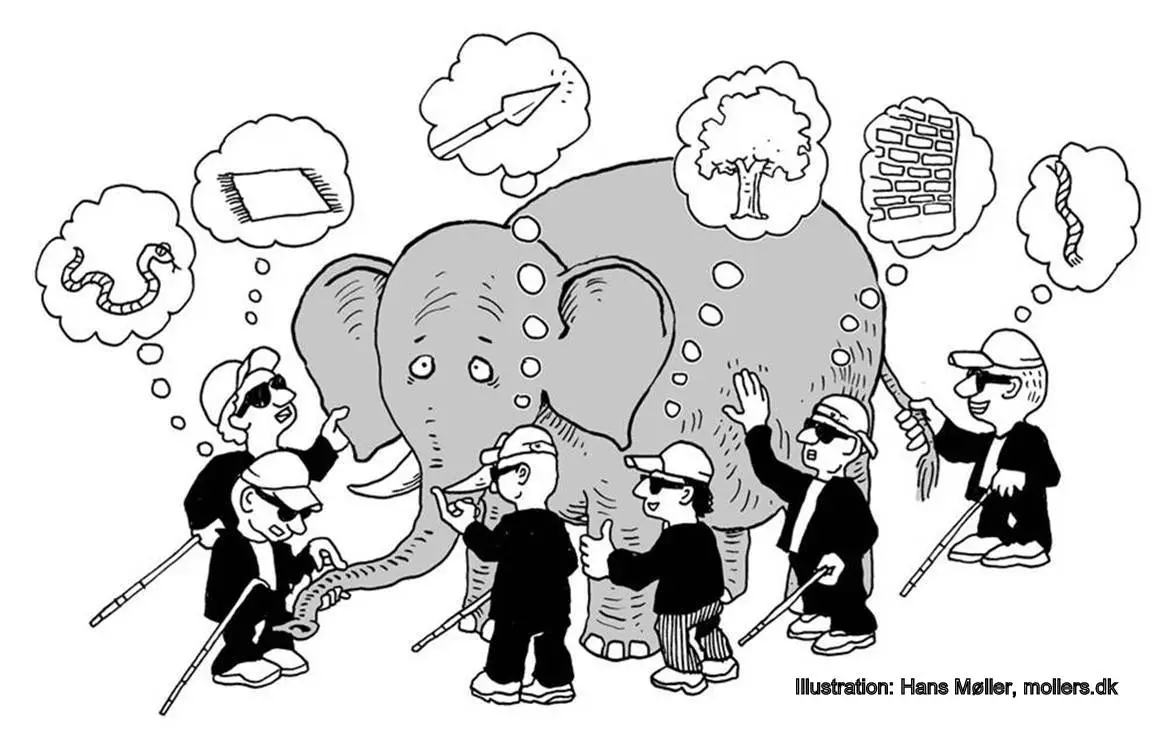
\includegraphics[width=16.17in]{Unidad-I/elefante} 

}

\caption{La parábola de los seis hombres ciegos inspeccionando un elefante.}\label{fig:unnamed-chunk-12}
\end{figure}

Quien toque los colmillos podrá pensar que se trata de una lanza, la trompa podría tratarse de una serpiente, la cola de una cuerda, las patas troncos de árbol y el cuerpo una pared. Es evidente que todas las hipótesis presentadas después de la inspección fueron erróneas, y que cuando estudiamos al mundo lo haremos igual, con la descripción de tan sólo una fracción de éste. Un séptimo hombre que pregunte a los otros seis qué fue lo que vieron podría formarse una imágen más completa del \emph{sistema} para proponer otra hipótesis: se trata de un objeto grande reposando sobre cuatro columnas con apéndices adelante y atrás.

Al estudiar los sistemas ecológicos, al igual que los ciegos, no sabremos que estamos frente a un elefante. Los sistemas ecológicos, al igual que los elefantes, también tienen componentes interconectados, y nosotros los ecólogos somos como los hombres ciegos, sólo podemos observar ciertas partes de los ecosistemas. En nuestro trabajo entonces, aprender a identificar y proponer hipótesis sobre cómo funcionan los sistemas ecológicos.

Las hipótesis propuestas por los seis hombres representan modelos, es decir simplificaciones del mundo que nos ayudan a entenderlo. Los modelos matemáticos son simplificaciones formales del mundo utilizando otro lenguaje, las matemáticas \citep{haefner1998modeling}.

\hypertarget{cuxf3mo-construir-un-modelo}{%
\section{Cómo construir un modelo}\label{cuxf3mo-construir-un-modelo}}

¿Cómo se construye un modelo? Es una pregunta difícil de responder, pues difícilmente existe un sólo modo de hacerlo que funcione para \href{mailto:tod@s}{\nolinkurl{tod@s}}. Aquí voy a hablar de mi propia experiencia, y cómo aprendí a utilizar las matemáticas y estadística para entender los sistemas ecológicos. Los pasos generales que sigo son:

\begin{enumerate}
\def\labelenumi{\arabic{enumi}.}
\tightlist
\item
  Identificar el sistema y sus componentes
\item
  Crear un modelo conceptual, haciendo dibujos
\item
  Identificar las herramientas matemáticas disponibles para representar el modelo conceptual
\item
  Establecer objetivos claros y alcanzables
\item
  Proponer una serie de modelos alternativos
\item
  Determinar una estrategia para seleccionar uno solo de los modelos que propuse para logar el objetivo
\end{enumerate}

\begin{figure}

{\centering 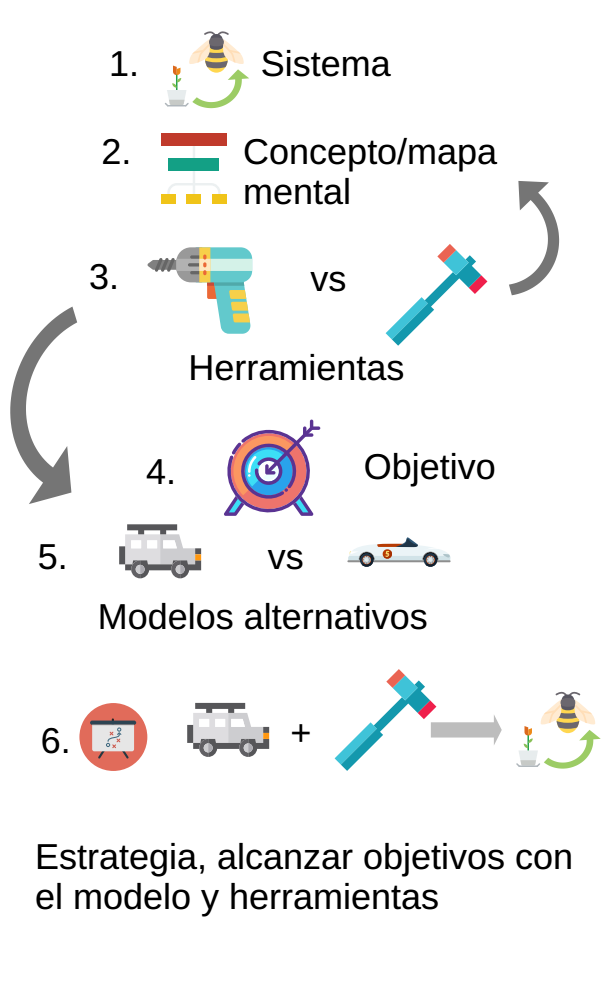
\includegraphics[width=8.5in]{Unidad-I/Diagrama-dearrollo} 

}

\caption{ Diagrama de mi estrategia para desarrollar modelos.}\label{fig:unnamed-chunk-13}
\end{figure}

La estrategia general que les doy puede, por el momento, sonar un tanto abstracta, pero la iremos poniendo en práctica conforme avanza el curso para que al final, esperemos, tenga más sentido que ahorita.

\hypertarget{ejemplos}{%
\subsection{Ejemplos}\label{ejemplos}}

La presente pandemia ha puesto en boca de todxs muchos aspectos de la modelación matemática y estadística. Como es de esperarse, los modelos son distintos dependiendo del objetido que se quiera conseguir con ellos:

\begin{enumerate}
\def\labelenumi{\arabic{enumi}.}
\tightlist
\item
  Determinar el número reproductivo básico (\(R_0\)) de COVID-19
\item
  Predecir la ocupación hospitalaria ante ciertas medidas de restricción de movilidad
\item
  Estimar cómo cambiaría el número reproductivo básico ante ciertas medidas de restricción
\item
  Predecir localidades geográficas donde surgirán nuevas cepas
\item
  Predecir las cualidades infecciosas o virulentas de las nuevas cepas
\end{enumerate}

Todos estos objetivos puede de cierta manera conseguirse por medio de modelos matemáticos, todos ellos con modelos muy distintos, algunos con herramientas muy diferentes unos de otros.

\hypertarget{discusiuxf3n-sobre-las-distintas-herramientas-matemuxe1ticas-empleadas-en-la-modelaciuxf3n-matemuxe1tica}{%
\section{Discusión sobre las distintas herramientas matemáticas empleadas en la modelación matemática}\label{discusiuxf3n-sobre-las-distintas-herramientas-matemuxe1ticas-empleadas-en-la-modelaciuxf3n-matemuxe1tica}}

Las matemáticas son un área de conocimiento muy extenso, por lo que hablar de todas las herramientas disponibles ¡nos podría llevar años! En este curso nos vamos a enfocar en un tipo general de modelo y de sistema ecológico: aquellos que cambian rápidamente con el tiempo, también llamados dinámicos.

Las herramientas matemáticas más comunmente utilizadas para estudiar estos sistemas son las ecuaciones diferenciales ordinarias y el álgebra de matrices. Las ecuaciones diferenciales nos ayudan a medir los cambios que sufre el sistema ecológico a través del tiempo en cada uno de sus componentes, y son muy útiles para representar las ideas plasmadas en forma de modelos conceptuales. El álgebra de matrices, por otro lado, nos sirve para \emph{conectar} los cambios de los diferentes componentes del sistema de estudio, y así hacer cálculos sobre sus cambios \emph{como un todo}.

Como podemos ver, gran parte de este curso estará enfocado en \emph{entender y medir los cambios}. Te preguntarás entonces ¿cambios de qué? En ecología, estos son algunos de los cambios que nos interesa observar:

\begin{enumerate}
\def\labelenumi{\arabic{enumi}.}
\tightlist
\item
  Número de individuos de una especie
\item
  Cantidad de materia orgánica almacenada en la vegetación
\item
  Calorías consumidas por una población de aves
\item
  Probabilidad de extinción de una especie
\end{enumerate}

\hypertarget{uso-de-los-modelos-matemuxe1ticos-en-ecologuxeda}{%
\section{Uso de los modelos matemáticos en ecología}\label{uso-de-los-modelos-matemuxe1ticos-en-ecologuxeda}}

Como ya mencionamos anteriormente, una alta proporción de las publicaciones académicas en ecología utiliza modelos matemáticos para predecir. Existen sin embargo otros usos de los modelos matemáticos que se pueden describir en términos generales como analíticos, es decir para analizar y entender cómo los diferentes componentes de un sistema afectan su coportamiento. Otras veces, los modelos se utilizan para medir las respuestas del sistema de interés ante perturbaciones, haciendo muchas simulaciones. Veamos una serie de ejemplos de estos diferentes usos de los modelos.

\hypertarget{analuxedticos-dinuxe1micas-depredador-presa}{%
\subsection{Analíticos: Dinámicas depredador-presa}\label{analuxedticos-dinuxe1micas-depredador-presa}}

En 1928, Vito Volterra \citep{volterra1928variations} desarrolló un modelo matemático para describir cómo varía el número de individuos de una especie de depredador y una presa. Como ya es conocido, este modelo replica muy bien el comportamiento oscilatorio de ambas poblaciones (Figura \ref{fig:volterra}).

\begin{figure}

{\centering 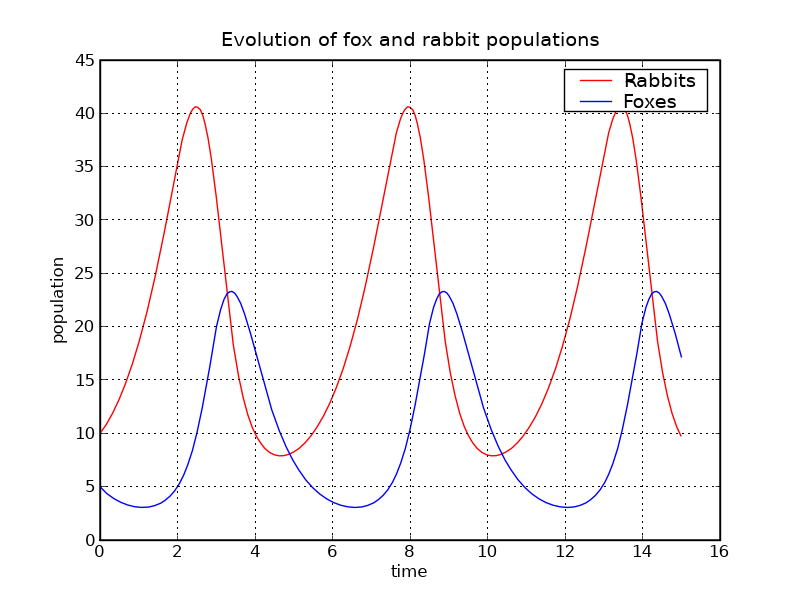
\includegraphics[width=11.11in]{Unidad-I/volterra} 

}

\caption{Simulación del modelo [Lotka-Volterra](https://scipy-cookbook.readthedocs.io/items/LoktaVolterraTutorial.html).}\label{fig:volterra}
\end{figure}

El comportamiento oscilatorio resulta \emph{obvio} desde una perspectiva biológica: los depredadores no se pueden reproducir a menos que se alimenten de sus presas, pero cuando hay muchos depredadores, estos consumen las presas disminuyendo sus números, resultando en menor potencial reproductivo para el depredador. Pero matemáticamente, ¿qué hace posible estas oscilaciones? Para responder esta pregunta se necesita entender bajo qué condiciones el sistema de ecuaciones que describe el sistema es estable, es decir cuándo los cambios de ambas poblaciones son cero, es decir bajo qué situaciones el sistema como un todo no experimenta cambio alguno. Este análisis matemático tiene un resultado un tanto sorprendente, pues las condiciones bajo las que dicha condición ocurre son un número imaginario, lo que indica que el sistema como tal es inestable, y por lo tanto \textbf{siempre} tiende a oscilar. El análisis de matemático de los modelos es en su mayoría netamente simbólico y requiere de buenas bases matemáticas.

\hypertarget{simulaciones-dinuxe1mica-de-enfermedades-infecciosas}{%
\subsection{Simulaciones: Dinámica de enfermedades infecciosas}\label{simulaciones-dinuxe1mica-de-enfermedades-infecciosas}}

Los sistemas ecológicos pueden ser muy complejos, lo que resulta en sistemas de ecuaciones igualmente complejos con muchas variables de estado y parámetros, y a la vez hace que el análisis sea muy complicado o imposible. En vista de ello se puede entonces \emph{resolver} el modelo utilizando herramientas computacionales. Un ejemplo que me gusta mucho es el estudio de la leptospirosis (infección por bacteria del género \emph{Leptospira}) en ratones \emph{Mastomys} de \citet{holt2006model}. Los autores formularon un modelo relativamente simple de ecuaciones diferenciales para ver cómo las constantes de su modelo afectan el número de ratones \emph{Mastomys} y de bacterias \emph{Leptospira} en el ambiente. Ello lo consiguieron aumentando en 10\% los valores de cada una de las constantes y midiendo el cambio tras cada simulación.

\begin{figure}

{\centering 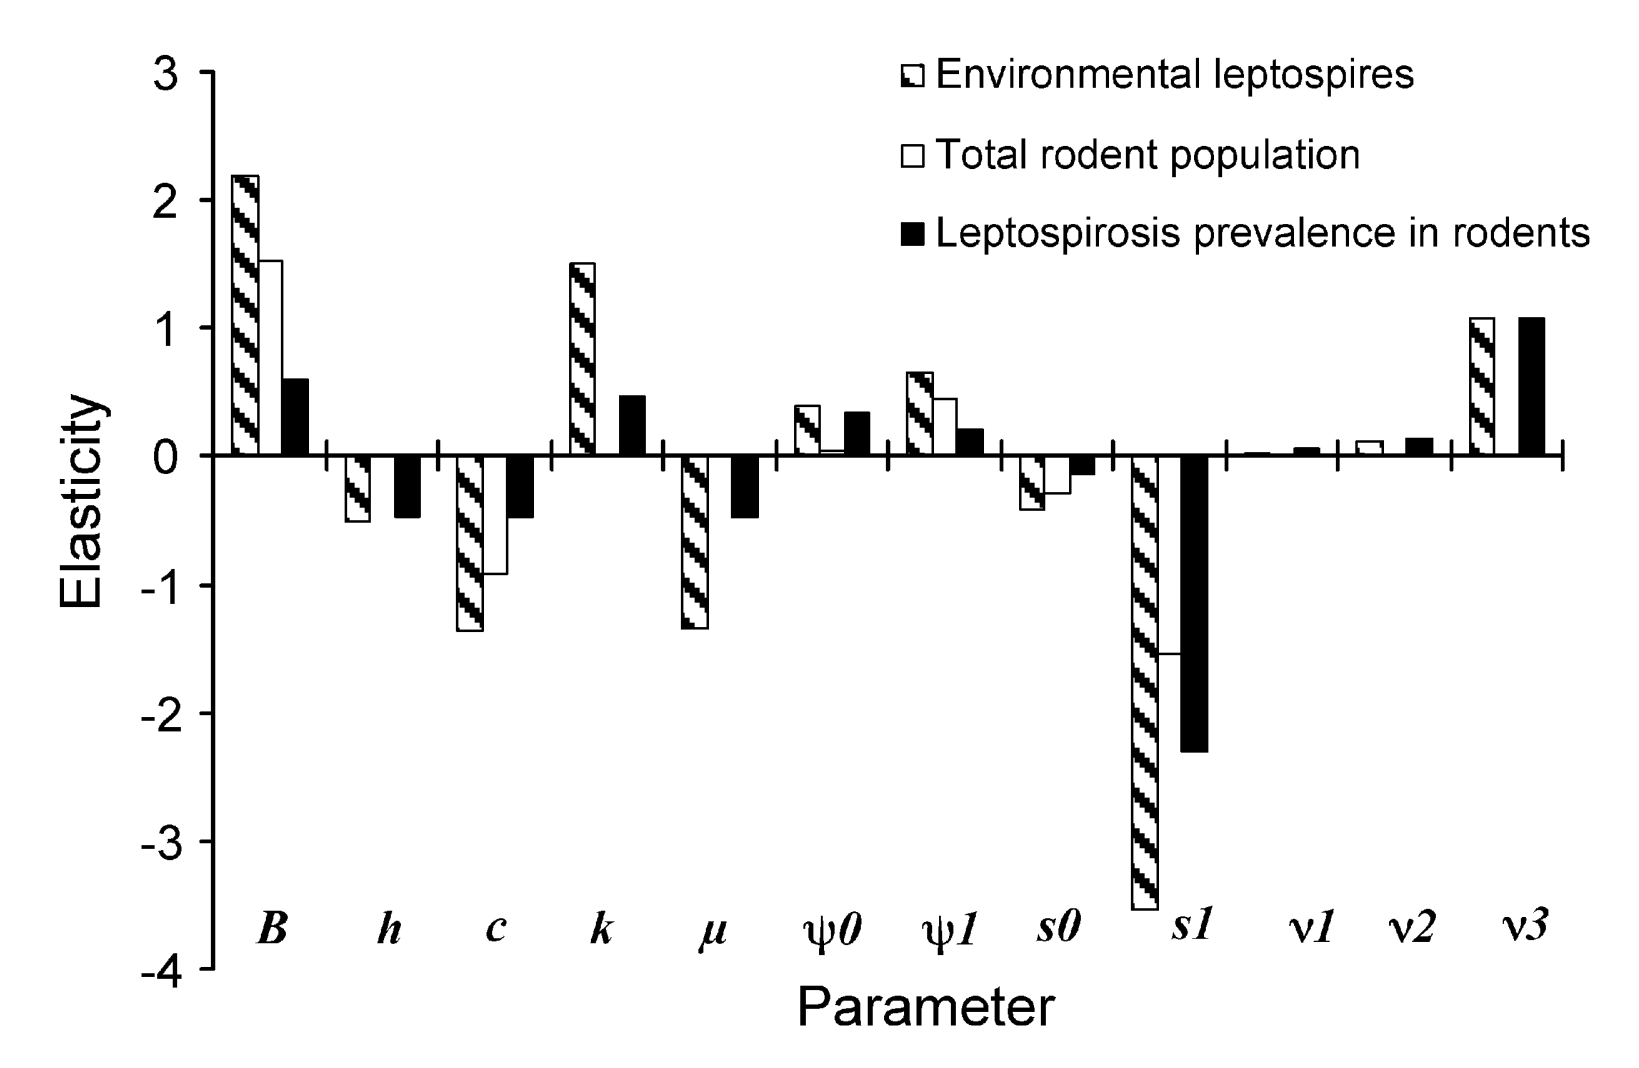
\includegraphics[width=22.78in]{Unidad-I/lepto} 

}

\caption{Las barras (eje $y$) indican el cambio proporcional de las diferentes cantidades de interés (color de las barras), ante el aumento del valor de cada parámetro (eje $x$), [@holt2006model].}\label{fig:lepto}
\end{figure}

Los análisis de sensibilidad mostrados en la Figura \ref{fig:lepto} son en realidad una serie de predicciones del sistema. De hecho la predicción generalmente echa mano de modelos matemáticos, así que nos centraremos en resumir: la predicción requiere de la planeación de una serie de escenarios para identificar áreas de intervención (alteración del hábitat por ejemplo) para obtener un resultado favorable de acuerdo con el modelo.

\hypertarget{mal-uso-de-los-modelos}{%
\subsection{Mal uso de los modelos}\label{mal-uso-de-los-modelos}}

Así como existe un uso adecuado de los modelos, es muy fácil darles un mal uso, generalmente relacionado con la calidad de los datos que los respaldan, el grado de entendimiento del sistema en cuestión, y con la relación entre las herramientas matemáticas utilizadas y la naturaleza del problema. \citet{holling1978adaptive} y \citet{karplus1975place}, sumarizan los siguientes usos potenciales de los modelos en relación a la calidad de los datos (1-baja calidad, 6-alta calidad):

\begin{enumerate}
\def\labelenumi{\arabic{enumi}.}
\tightlist
\item
  Atención del público
\item
  Aprendizaje sobre el sistema
\item
  Prueba de teorías
\item
  Juegos ``qué pasaría si\ldots{}''
\item
  Recomendación de acciones
\item
  Diseño de productos
\end{enumerate}

\hypertarget{tipos-de-modelos}{%
\section{Tipos de modelos}\label{tipos-de-modelos}}

La clasificación de los modelos depende de la herramienta que se utiliza para desarrollarlos. En la sección ``Cómo construir un modelo'', mencioné brevemente que uno de los pasos es la formulación de un modelo ``conceptual'', en forma de un esquema o diagrama. Esta clasificación la podemos ampliar un poco:

\begin{enumerate}
\def\labelenumi{\arabic{enumi}.}
\tightlist
\item
  \textbf{Modelo conceptual o verbal}. Descripciones en lenguaje natural.
\item
  \textbf{Diagramático}. Representación gráfica (diagramas de flujo o cajas).
\item
  \textbf{Físico}. Representación a escala de sistema (sistemas hidráulicos).
\item
  \textbf{Formal}. Matemático (algebráico o sistemas de ecuaciones).
\end{enumerate}

Aquí nos centraremos en ver a mayor profundidad los modelos formales, en clasificar los modelos matemáticos. \citet{haefner1998modeling} sugiere la siguiente clave dicotómica de clasificación:

\begin{enumerate}
\def\labelenumi{\arabic{enumi}.}
\item
  \textbf{¿Las matemáticas representan de manera explícita el proceso de interés?}

  1.1. \textbf{Sí}: Modelo mecanístico

  1.2. \textbf{No}: Modelo descriptivo, fenomenológico
\item
  \textbf{¿Las matemáticas representan de manera explícita las condiciones del estado futuro del sistema?}

  2.1. \textbf{Sí}: Modelo dinámico

  2.2. \textbf{No}: Modelo estático
\item
  \textbf{¿Las matemáticas representan el tiempo de manera contínua?}

  3.1. \textbf{Sí}: Modelo conínuo

  3.2. \textbf{No}: Modelo discreto (el tiempo sólo toma valores enteros, un día, un año)
\item
  \textbf{¿Las matemáticas representan explícitamente el espacio?}

  4.1. \textbf{Sí}: Modelo espacialmente heterogéneo

  4.2. \textbf{No}: Modelo espacialmente homogéneo
\item
  \textbf{¿Las matemáticas permiten la ocurrencia de eventos aleatorios?}

  5.1. \textbf{Sí}: Modelo estocástico

  5.2. \textbf{No}: Modelo determinístico
\end{enumerate}

\hypertarget{ejemplos-1}{%
\subsection{Ejemplos}\label{ejemplos-1}}

\hypertarget{modelo-de-presa-depredador-de-el-modelo-de-lotka-volterra--volterra1928variations}{%
\subsubsection{\texorpdfstring{Modelo de presa-depredador de El modelo de Lotka-Volterra \citeyearpar{volterra1928variations}}{Modelo de presa-depredador de El modelo de Lotka-Volterra {[}-@volterra1928variations{]}}}\label{modelo-de-presa-depredador-de-el-modelo-de-lotka-volterra--volterra1928variations}}

\begin{figure}

{\centering 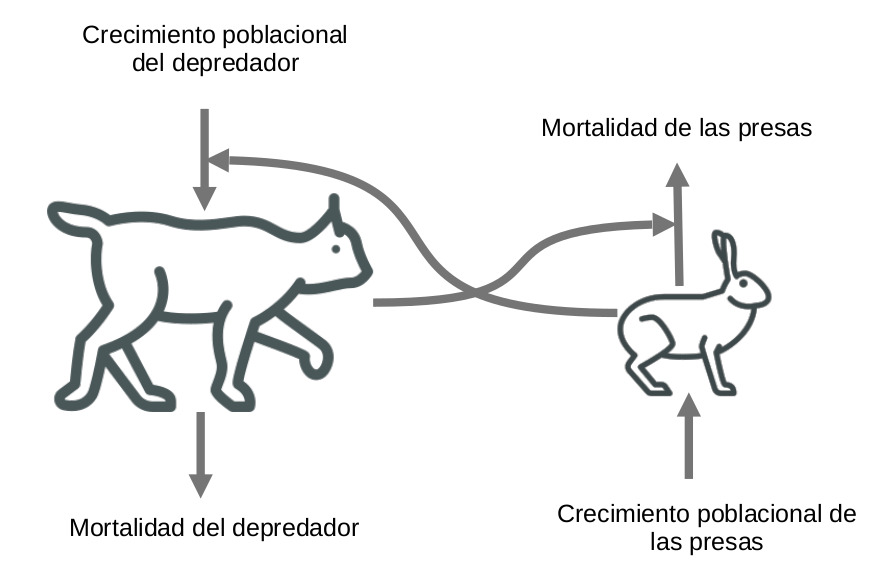
\includegraphics[width=12.18in]{Unidad-I/Volterra/Volterra} 

}

\caption{Modelo diagramático basado en el modelo matemático depredador-presa de Lotka-Volterra}\label{fig:volterra-diag}
\end{figure}

Este modelo representa cómo cambia el número de liebres y linces a través del tiempo con un sistema de ecuaciones diferenciales. El cambio en los números de individuos depdende de

\begin{enumerate}
\def\labelenumi{\arabic{enumi}.}
\tightlist
\item
  Crecimiento poblacional del depredador en relación a las presas disponibles para que el depredador se alimente
\item
  Crecimiento poblacional innato de las presas
\item
  Mortalidad de presas en relación a la cantidad de depredadores
\item
  Mortalidad innata del depredador
\end{enumerate}

El modelo entonces representa el mecanismo del sistema, por lo que es un modelo \textbf{mecanístico}. Debido a que representa el cambio del número de individuos en el tiempo, es un modelo \textbf{dinámico}. Por el momento no contamos con información suficiente para decir si es contínuo o discreto, pero no hay mención del componente espacial, por lo que podemos suponer que se trata de un modelo \textbf{espacialmente homogéneo}. La solución al modelo clásico de la figura \ref{fig:volterra-diag}, muestra un patrón regular, lo cual se debe a que todos los parámetros son constantes, y por lo tanto es un modelo \textbf{determinista}.

\hypertarget{modelo-del-panal-de-abejas}{%
\subsubsection{Modelo del panal de abejas}\label{modelo-del-panal-de-abejas}}

\citet{wilenski2003honey} desarrolló un modelo para representar cómo las abejas construyen un panal, por medio de una serie de reglas que rigen el comportamiento de abejas individuales. Debido a que el mecanismo está representado en el comportamiento colectivo de las abejas, es un modelo \textbf{mecanístico}. El modelo también muestra la progresión de la construcción del panal, por lo que es un modelo \textbf{dinámico}, y debido a que cualquiera de los eventos posibles pueden ocurrir en cualquier momento es en tiempo \textbf{contínuo}. También representa la estructura del panal en unidades espaciales, por lo que es \textbf{espacialmente heterogéneo}. Finalmente, los eventos que ocurren son aleatorios, o sea que el resultado de una realización del modelo será diferente de otra, por lo que es un modelo \textbf{estocástico}. Te invito a explorar este modelo por medio de la aplicación en línea de \href{https://www.netlogoweb.org/launch\#https://www.netlogoweb.org/assets/modelslib/Sample\%20Models/Biology/Honeycomb.nlogo}{NetLogo}.

A continuación veremos a mayor profundidad los modelos deterministicos y estocásticos.

\hypertarget{modelos-determinuxedsticos-y-estocuxe1sticos}{%
\subsection{Modelos determinísticos y estocásticos}\label{modelos-determinuxedsticos-y-estocuxe1sticos}}

Imaginemos que necesitamos un librero, y para ello necesitamos medir las dimensiones del espacio donde lo colocaremos. Solamente contamos con una cinta en pulgadas, pero el carpintero, para hacer el presupuesto, necesita las medidas en centímetros. Entonces para hacer la conversión de pulgadas a centímetros utilizamos el siguiente modelo:

\begin{equation}
    cm = 2.54 \times in  \label{eq:pulgadas}
\end{equation}

donde \(in\) son las pulgadas, \(cm\) los centímetros, y \(2.54\) es la constante de conversión. Entonces ya tenemos así un modelo que siempre nos dará la misma respuesta para cada valor de entrada:

\begin{itemize}
\tightlist
\item
  \(2in \rightarrow 2 \times 2.54cm = 5.08cm\)
\item
  \(11in \rightarrow 11 \times 2.54cm = 27.94cm\)
\end{itemize}

Imaginemos ahora que la constante de conversión no fuera una sola, \(2.54\), sino cientos, o miles de posibles valores cercanos a \(2.54\), y cada vez que resolvemos el modelo \eqref{eq:pulgadas} obtenemos un valor distinto. El primero es un modelo deterministico, siempre da la misma respuesta. El segundo, es un modelo estocástico. Te preguntarás entonces ¿para qué querríamos un modelo que de respuestas inconsistentes? La principal razón es que en ecología, como en otras áreas del conocimiento, los sistemas de estudio son muy variables, y los modelos estocásticos nos sirven para representar esa variabilidad y conocer algunos de los posibles resultados. En pocas palabras, si un sistema es determinista, siempre podemos conocer su comportamiento con alta precisión, mientras que en los estocáticos, no.

\hypertarget{deterministicos}{%
\subsubsection{Deterministicos}\label{deterministicos}}

En vista de mi comentario ``\ldots{} los sistemas de estudio son muy variables\ldots{}'' tal vez te surja otra pregunta, ¿entonces por qué estudiamos los modelos deterministas? Y no hay una pregunta mmuy sencilla, pero la principal es que son más sencillos. Por otra parte, si pensamos en los modelos desde un punto de vista estadístico, se podría también sugerir que podemos utilizar los modelos determinísticos para estudiar el comportamiento ``promedio'', o para caracterizar ese componente, el determinista, de nuestro sistema de estudio. En este sentido, se considera entonces que la mayoría de los sistemas y procesos ecológicos tienen un componente determinístico y uno estocástico. La mejor manera de modelar los sistemas ecológicos, entonces, es utilizando ambos. Por lo tanto, para modelar los sistemas ecológicos con ambos métodos, necesitamos aprender a utilizarlos por separado.

Una de las grandes bondades de los modelos determinísticos es que nos permiten analizar el comportamiento del sistema de estudio. Los modelos de cambio temporal, por ejemplo, han sido muy importantes en el desarrollo de la teoría del caos, la cual sirve para explicar por qué ciertos procesos del mundo natural nunca alcanzan un nivel de estabilidad (¡dinámicas depredaror-presa!).

\hypertarget{estocuxe1sticos}{%
\subsubsection{Estocásticos}\label{estocuxe1sticos}}

A diferencia de los modelos deterministas, los estocásticos nunca dan el mismo resultado. Existe un gran variedad de herramientas computacionales y formulaciones matemáticas para conseguir este tipo de comportamiento. En la mayoría de los casos, los modelos deterministas constan de dos componentes, uno determinista, relacionado con los mecanismos propios del sistema de estudio, y uno aleatorio, encargado de generar los eventos posibles o de simular la variación en el componente determinista. Esto lo podemos ilustrar con el modelo de conversión de pulgadas a centímetros:

\[
cm = 2.54 \times in
\]
el cual es determinista. Sin embargo, podemos formular una versión estocástica, que añada una pequeña cantidad a la conversión determinística cada vez que la calculamos:

\[
cm = 2.54 \times in + \varepsilon
\]

donde \[\varepsilon\] es el \emph{error} que hemos introducido. Técnicamente para hacer esto utilizamos un generador de números aleatorios en el lenguaje de programación \textbf{R}. Veamos una serie de conversiones:

\begin{table}

\caption{\label{tab:unnamed-chunk-16}Cinco realizaciones para la conversión de dos pulgadas a centímetros con el modelo determinista y estocástico.}
\centering
\begin{tabular}[t]{c|c}
\hline
Determinista & Estocástico\\
\hline
5.08 & 5.351191\\
\hline
5.08 & 5.392189\\
\hline
5.08 & 5.166747\\
\hline
5.08 & 5.267774\\
\hline
5.08 & 5.114500\\
\hline
\end{tabular}
\end{table}

Este tipo de \emph{inconsistencias} de los modelos estocásticos tienen implicaciones muy importantes para el comportamiento de modelos como el de Lotka-Volterra, que veremos más adelante.

\hypertarget{unidad-ii-introducciuxf3n-a-los-modelos-determinuxedsticos}{%
\chapter{Unidad II: Introducción a los modelos determinísticos}\label{unidad-ii-introducciuxf3n-a-los-modelos-determinuxedsticos}}

\hypertarget{la-luxednea-recta}{%
\subsection{La línea recta}\label{la-luxednea-recta}}

Una línea recta se puede representar matemáticamente de varias maneras, la más común de ellas es por medio de una función. Una función, en cambio es una expresión matemática que indica una serie de operaciones (aritméticas por ejemplo), que serán aplicadas a un conjunto de números en sucesión (los números reales, p.~ej.) para producir otro conjunto. Así la, función lineal más sencilla puede ser:

\begin{equation}
    y(x) = x
\end{equation}

Lo que quiere decir que \(y\) es una función de \(x\), y cada valor de \(y\) será igual a cada valor de \(x\). En lenguaje matemático, el conjunto de números de \(x\) se llama el dominio, y \(y(x)\) el codominio. Algunas funciones lineales más complejas son:

\begin{equation}
    y(x) = ax
\end{equation}

donde \(a\) es una constante, lo que quiere decir que cada valor de \(y(x)\) será producido por el producto \(a \times x\). Finalmente, la expresión más común de una ecuación lineal es:

\begin{equation}
    y(x) = b + ax
\end{equation}

donde \(b\) también es una constante que se llama intercepto, y \(a\) es la pendiente, pues esta última determina la inclinación de la línea recta representada en el plano cartesiano.

\hypertarget{representaciones-gruxe1ficas-de-la-recta}{%
\subsubsection{Representaciones gráficas de la recta}\label{representaciones-gruxe1ficas-de-la-recta}}

Comencemos por dar un repaso del plano cartesiano. Este consiste de la representación de dos conjuntos de números reales en los que representamos una función, como una regla de correspondencia entre los valores de cada conjunto, de modo que a cada valor de \(x\) corresponde uno y sólo uno de los valores de \(y\). Cada conjunto se puede representar como una recta, y cuando éstas se disponen perperdiculares dan origen al plano.

\begin{figure}

{\centering 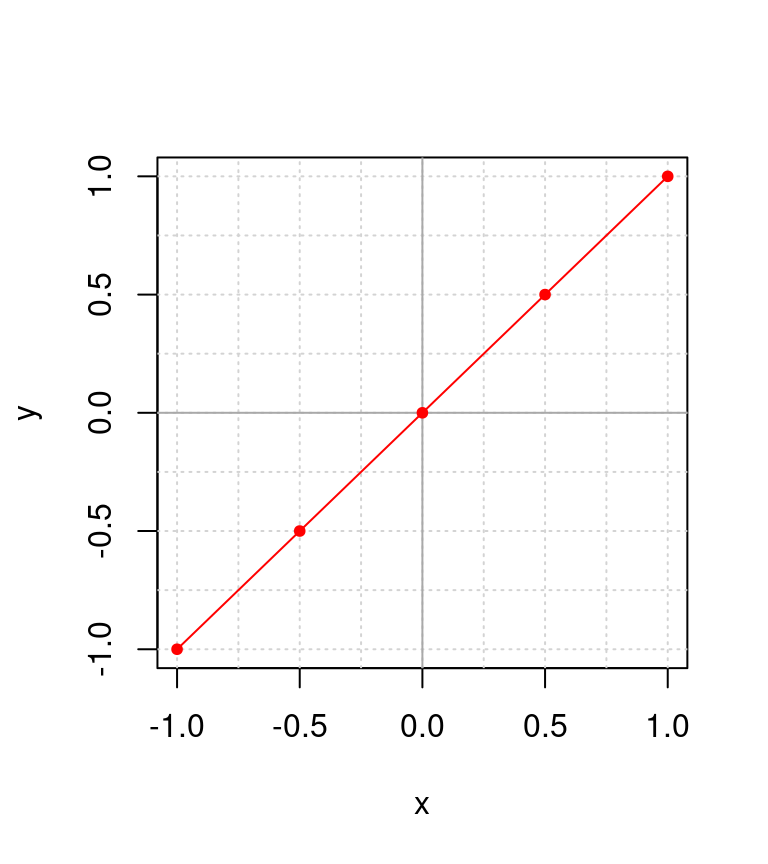
\includegraphics{Mod-mat-ECO_files/figure-latex/unnamed-chunk-17-1} 

}

\caption{Ejemplo del plano cartesiado mostrando en rojo la correspondencia de valores para $y(x) = x$, donde los puntos corresponden a los pares de valores $(x = -1, y = -1), (-0.5, -0.5), (0, 0), (0.5, 0.5), (1, 1)$.}\label{fig:unnamed-chunk-17}
\end{figure}

Ahora veamos, con un ejemplo gráfico por qué la constante \(a\) recibe el nombre de \emph{pendiente}.

\begin{figure}

{\centering 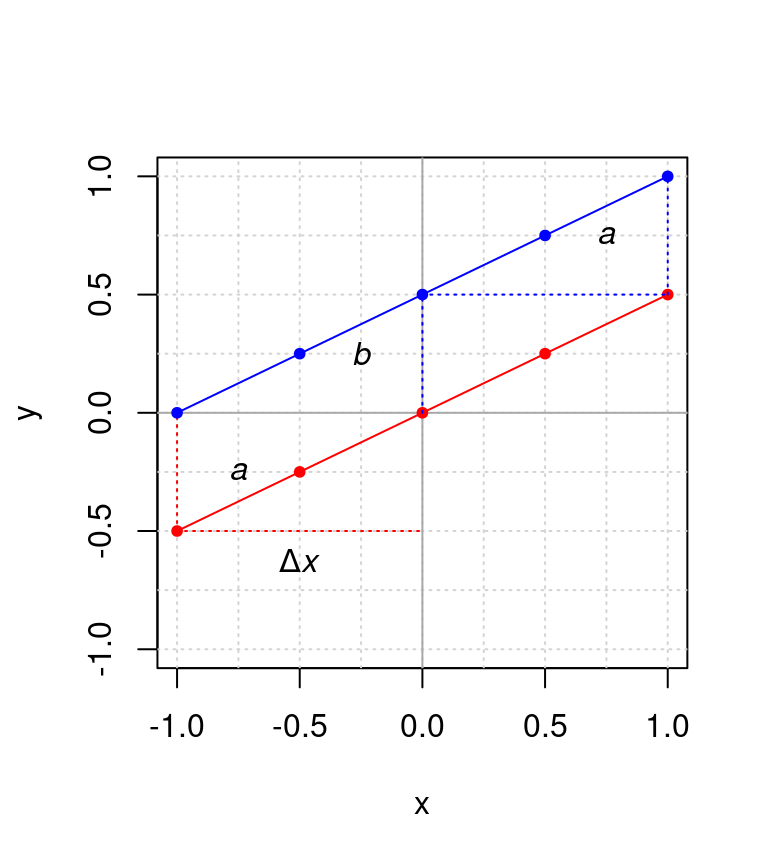
\includegraphics{Mod-mat-ECO_files/figure-latex/unnamed-chunk-18-1} 

}

\caption{Gráficas de las funciones $y(x) = 0.5 x$ (en rojo) y $y(x) = 0.5 + 0.5 x$ (azul). Las líneas punteadas en colores indican el efecto de las constantes $a$ y $b$, mientas que Δ$x$ denota el cambio de una unidad de $x$.}\label{fig:unnamed-chunk-18}
\end{figure}

Como podemos ver, de manera más general, la línea recta es generada por una regla de correspondencia muy sencilla, un conjunto de valores \(X\) son multiplicados por un escalar \(a\), a los que se les puede añadir un \emph{intercepto} \(b\). El intercepto siempre es el valor de \(y(x)\) cuando \(x = 0\).

Ya se podrán imaginar que puede existir un sinnúmero de modelos lineales distintos, por ejemplo si \(y\) es una función de un gran número de conjuntos \(X\):

\begin{equation}
y(x_1, x_2, \dots, x_{n-1}, x_n) = b + a_1 x_1 + a_2 x_2 + \dots + a_{n-1} x_{n-1} + a_n x_n
\end{equation}

Gráficamente, estamos prácticamente limitados a explorar \(y(x_1, x_2)\), pero existen muchas herramientas matemáticas para entender modelos lineales más complejos que veremos más adelante. Estas herramientas y las implicaciones generales de la simplicidad del modelo lineal lo hacen uno de los modelos más útiles con que contamos para estudiar matemáticamente fenómenos dinámicos (que cambian de estado a lo largo del tiempo), como para estudiarlos de manera probabilística (con estadística). De hecho, el modelo lineal nos puede servir para entender modelos, como la parábola y el exponencial, que geométricamente no se parecen a la línea recta.

\hypertarget{la-paruxe1bola}{%
\subsection{La parábola}\label{la-paruxe1bola}}

Geométricamente, la parábola es muy distinta de la recta:

\begin{figure}

{\centering 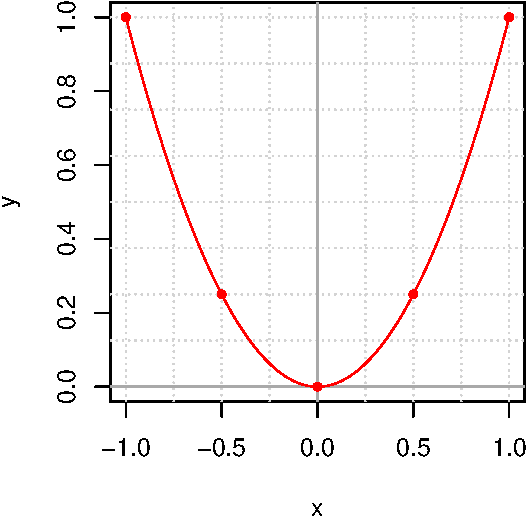
\includegraphics{Mod-mat-ECO_files/figure-latex/parabola-1} 

}

\caption{Ejemplo del plano cartesiado mostrando en rojo la correspondencia de valores para $y(x) = x^2$, donde los puntos corresponden a los pares de valores $(x = -1, y = 1), (-0.5, 0.25), (0, 0), (0.5, 0.25), (1, 1)$.}\label{fig:parabola}
\end{figure}

La función matemática más sencilla que puede describir esta forma en el plano cartesiano es:

\begin{equation}
    y(x) = x^2
\end{equation}

Al igual que con los modelos lineales, las parábolas pueden representarse matemáticamente de otras formas más complejas:

\begin{itemize}
\tightlist
\item
  \(y(x) = a + bx + cx^2\)
\item
  \(y(x) = a + cx^2\)
\item
  \(y(x) = -x^2\)
\end{itemize}

Si uno es observador, se dará cuenta de que estas ecuaciones son muy similares a la recta, y es que es posible considerar que \(x^2\) se puede considerar como otro conjunto tal que \(x' = x^2\), resultando así en funciones perferctamente lineales:

\begin{itemize}
\tightlist
\item
  \(y(x) = a + bx + cx'\)
\item
  \(y(x) = a + cx'\)
\item
  \(y(x) = -x'\)
\end{itemize}

Entonce, lo que realmente distingue matemáticamente a una parábola de una recta, es la doble ocurrencia de cada valor de \(y\) para los distintos valores de \(x\):

\begin{figure}

{\centering 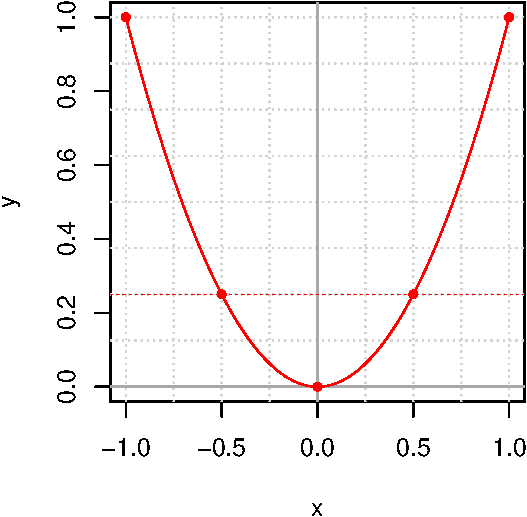
\includegraphics{Mod-mat-ECO_files/figure-latex/parabola-2-1} 

}

\caption{Correspondencia de dos valores distintos de $x$ para el mismo valor de $y$}\label{fig:parabola-2}
\end{figure}

Cuando esto ocurre, las funciones tiene un solo punto a lo largo de todos los valores de \(x\), donde sólo va a ocurrir un valor único de \(y\). A estos puntos se les conocen como mínimos (par de valores con coordenadas \((0, 0)\) en la figura \ref{fig:parabola-2}). Los máximos, en cambio están ilustrados en la figura \ref{fig:parabola-3}, e igual corresponde al punto con coordenadas \((0, 0)\).

\begin{figure}

{\centering 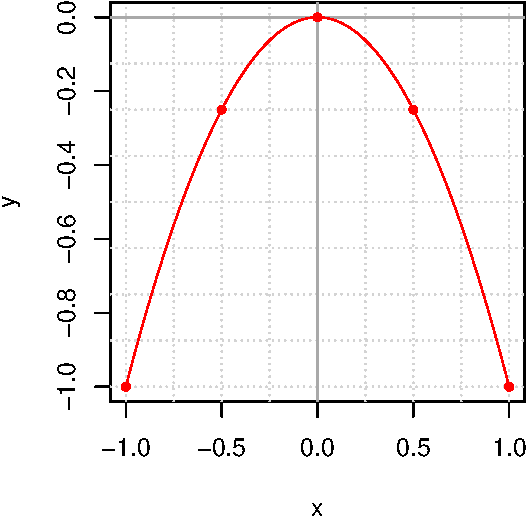
\includegraphics{Mod-mat-ECO_files/figure-latex/parabola-3-1} 

}

\caption{Correspondencia de valores para $y = -x^2$.}\label{fig:parabola-3}
\end{figure}

En los modelos parabólicos más sencillos (\(y(x) = x^2, y(x) = -x^2\)), los puntos mínimos y máximos siempre estarán en las coordenadas \((x = 0, y = 0)\), pero es posible alterarlos. Por ejemplo en \(y(x) = 2 + x^2\), el mínimo estará en \((x = 0, y = 2)\). Para verificarlo resuelve \(y(x) = 2 + x^2\) para \(y(0)\), sustituyendo \(x\) por \(0\).

\hypertarget{ejercicio}{%
\subsubsection{Ejercicio}\label{ejercicio}}

A estas alturas, ya te podrás haber dado cuenta de ciertas propiedades de las parábolas, contesta las siguientes preguntas:

\begin{enumerate}
\def\labelenumi{\arabic{enumi}.}
\item
  ¿Qué tipo de punto único (mínimo o máximo) habrá en las siguientes parábolas?

  1.1. \(y(x) = 2 - x^2\)
  1.2. \(y(x) = 2x - 2x^2\)
  1.3. \(y(x) = 1 - x + 3x^2\)
  1.4. \(y(x) = x/2 - 4x^2/x\)
  1.5. \(y(x) = (5x)^2 - 3x + 1\)
\end{enumerate}

\hypertarget{cuxf3nicas}{%
\subsection{Cónicas}\label{cuxf3nicas}}

De manera muy general, una cónica es el conjunto de soluciones para una ecuación cuadrática cuando menos en dos variables. En este sentido, las parábolas, vistas en la sección anterior, son un tipo de cónica. Ejemplos:

\begin{enumerate}
\def\labelenumi{\arabic{enumi}.}
\tightlist
\item
  \(x^2 + y^2 = -1\)
\item
  \(x^2 + y^2 = 0\)
\item
  \(x^2 - y^2 = 0\)
\item
  \(xy - 1 = 0\)
\item
  \(x^2 - y = 0\)
\end{enumerate}

Debido a la generalidad de la definición de \emph{cónicas}, las ecuaciones 1-5 tienen una variedad de formas muy distintas, en comparación con las secciones de rectas y parábolas (Figura \ref{fig:conicas}). La mayoría de estas forman surgen como solución a la intersección de un plano bidimensional con una línea rotando sobre un eje definido dentro de ella en un espacio tridimencional (\href{https://www.mathplanet.com/Oldsite/media/28029/conic.png}{ver ejemplo})

\begin{figure}

{\centering 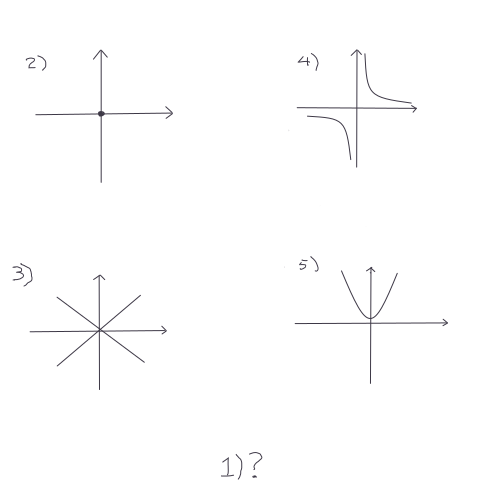
\includegraphics[width=6.93in]{Unidad-II/conicas} 

}

\caption{Representación gráfica de las ecuaciones 1-5.}\label{fig:conicas}
\end{figure}

\hypertarget{la-curva-normal}{%
\subsection{La curva normal}\label{la-curva-normal}}

En el curso de probabilidad y estadística, se acordarán, se mencionó repetidamente a la distribución normal. En cuestión de matemáticas, la distribución normal puede ser representada como una ecuación:

\begin{equation}
    y(x) = \frac{1}{\sigma \sqrt{2\pi}}e^{-\frac{(x-\mu)^2}{2\sigma^2}} \label{eq:normal}
\end{equation}

donde \(\mu\) es la media aritmética, \(\sigma^2\) es la varianza y \(x\) son todos los valores de la variable que observamos. Cuando tenemos datos de un experimento y los analizamos haciendo el cálculo del promedio estimamos justamente a \(\mu\) de la ecuación \eqref{eq:normal}, y al estimar la varianza obtenemos a \(\sigma^2\) de la misma ecuación. Como es importante notar, al hacer estos cálculos estamos asumiendo que nuestros datos tienen una distribución (un histograma) que puede ser descrita por la ecuación \eqref{eq:normal}.

Como vimos en la sección de parábolas, las funciones que no son monótonas (los valores de \(y\) no aumentan o disminuyen a lo largo de \(x\)), tienen un punto máximo o mínimo. La curva normal, tiene propiedades similares, aunque debido a la presencia de la función exponencial (\(e^{\dots}\)), los valores de \(y(x)\) \textbf{siempre serán positivos}. Por lo tanto, la curva normal tiene un punto máximo que corresponde a \(y(\mu)\), o sea, \(y\) alcanza su punto máximo cuando \(x=\mu\) (Figura \ref{fig:normal}).

\begin{figure}

{\centering 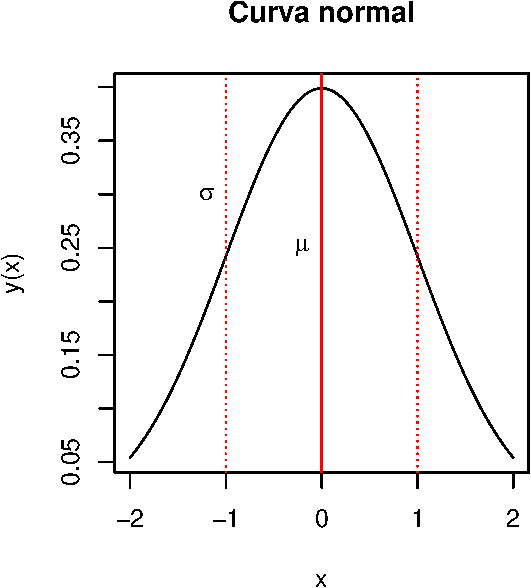
\includegraphics{Mod-mat-ECO_files/figure-latex/normal-1} 

}

\caption{Representación gráfica de la curva normal.}\label{fig:normal}
\end{figure}

En estadística, esta función representa en el eje de las \(y\) la \emph{densidad} de la variable \(x\). Densidad se refiere a la proporción de observaciones de \(x\) dentro de un intervalo definido de \(x\). Por lo tanto, la curva normal, representa la probabilidad de observar ese valor de \(x\), de ahí que \(\mu\) sea el valor teórico más probable. En lo que respecta a \(\sigma^2\), éste representa qué tan concentrados estarán los valores de \(x\) alrededor de \(\mu\). Altos valores de \(\sigma\) se traducirán en baja concentración alrededor de \(\mu\) (Figura \ref{fig:vari}).

\begin{figure}

{\centering 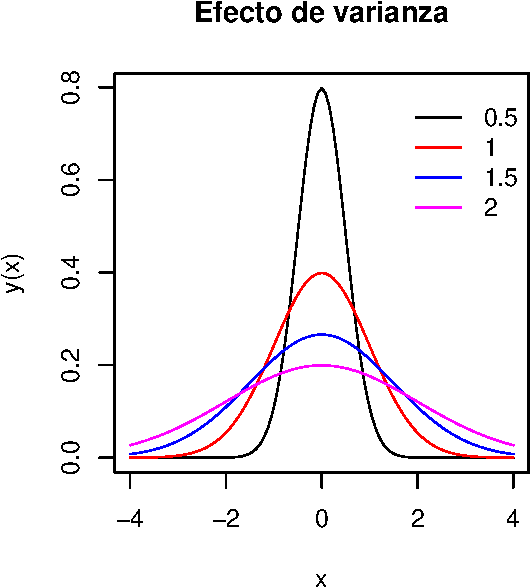
\includegraphics{Mod-mat-ECO_files/figure-latex/vari-1} 

}

\caption{Efecto de  la varianza sobre la la dispersión alrededor de la media.}\label{fig:vari}
\end{figure}

\hypertarget{unidad-iii---introducciuxf3n-al-cuxe1culo-diferencial-e-integral}{%
\chapter{Unidad III - Introducción al cáculo diferencial e integral}\label{unidad-iii---introducciuxf3n-al-cuxe1culo-diferencial-e-integral}}

  \bibliography{book.bib,packages.bib,citas.bib}

\end{document}
